\documentclass{standalone}
% Preamble
\begin{document}

\subsection{Structure bloc-triangulaire et rang numérique de $B(1)$}
Dans le processus de réduction, la première étape consiste à calculer le noyau de $B(1)$. Lorsque les coefficients des polynômes d'entrée sont entiers ou rationnels, ceci peut se faire de manière exacte au moyen d'un programme de calcul symbolique. La taille des entiers peut alors croître considérablement au cours des calculs et augmenter en conséquence le temps total de calcul et les besoins en mémoire du calculateur. Si par contre on veut effectuer l'ensemble des calculs en nombres flottants, ou si les coefficients d'entrée sont eux mêmes donnés sous forme numérique, alors on doit faire un calcul numérique du noyau. La méthode éprouvée pour cela, implémentée dans des packages d'algèbre linéaire numérique comme Matlab/Octave, Numpy ou Julia, est d'effectuer une factorisation QR ``rank revealing'' de $B(1)$, que nous appellerons factorisation QRP, c'est-à-dire accompagnée de pivots sur les colonnnes. L'expérience montre que cette approche est souvent efficace mais peut s'avérer délicate à mettre en oeuvre si la taille de la matrice augmente. Montrons le sur un exemple. Nous choisissons $n = 4$ et un système polynomial $f$ de multidegré $d = (2, 2, 2, 2)$. Chaque polynôme possède $m = 15$ monômes. Les degrés sont choisis aléatoirement suivant une loi uniforme entre $0$ et $2$. Les coefficients, entiers, sont choisis aléatoirement suivant une loi uniforme entre $-5$ et $5$. La matrice de Bezout $B(1)$ est de taille $384$ et on peut voir apparaitre une certaine structure, comme le montre la figure ci-dessous.
% \begin{wrapfigure}{r}{0.5\textwidth}
  \begin{center}
    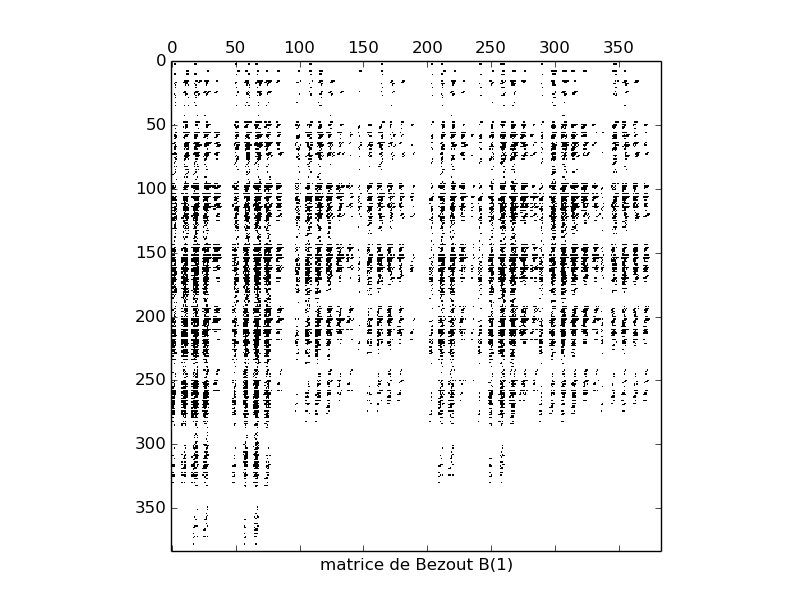
\includegraphics[width=0.48\textwidth]{../png/bez.png}
  \end{center}
% \end{wrapfigure}
Cependant il parait difficile d'exploiter cette structure pour le calcul du rang de la matrice $B(1)$. On doit donc avoir recours à une méthode numérique générale, par exemple une factorisation SVD ou une factorisation QRP ``rank revealing''. Choisissons cette deuxième méthode. Les termes diagonaux du facteur triangulaire $R$ seront triés en ordre décroissant, comme le montre la figure ci-dessous.
% \begin{wrapfigure}{l}{0.5\textwidth}
  \begin{center}
    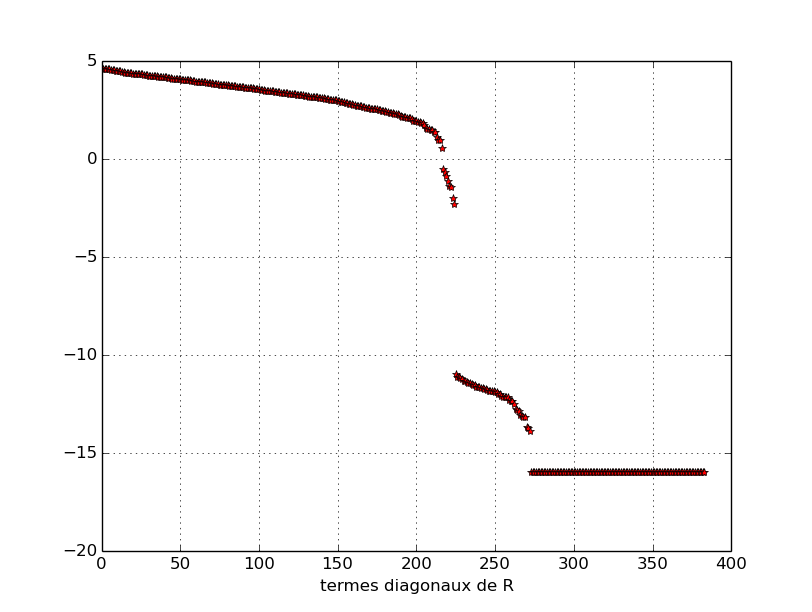
\includegraphics[width=0.48\textwidth]{../png/diagR.png}
  \end{center}
% \end{wrapfigure}
 On s'aperçoit que les derniers termes non nuls décroissent très vite, et qu'il peut devenir difficile de choisir un seuil au dessus duquel les termes diagonaux seront déclarés ``non nuls''. Le ``saut'' entre termes ``non-nuls'' et termes proches du epsilon machine a tendance à diminuer à mesure que la taille de la matrice augmente, ce qui rend le calcul du rang numérique difficile. Pour cet exemple, voici la table des termes de la diagonale entre les indices $294$ et $297$.
 $$
 \begin{array}{c|c}
 	i & \vert R_{i,i}\vert \\
 	\hline
 	294  & 1e-4 \\
 	295 & 1e-6 \\
 	296 & 1e-11 \\
 	297 & 1e-11 \\
 \end{array}
 $$
On constate qu'il est difficile, à partir de ces valeurs de fixer un seuil en dessous duquel les termes peuvent être considérés comme négligeables. On aurait tendance à fixer naturellement le seuil entre les indices $295$ et $296$ ce qui donne $295$ comme rang numérique de $B(1)$. C'est la valeur fournie par la fonction rank de numpy. Or $B(1)$ est une matrice à coefficients entiers et on peut donc calculer son rang exact au moyen d'un logiciel de calcul symbolique. Pour le logiciel Sage le rang de la matrice à coefficient entiers $B(1)$ vaut $296$, en contradiction avec la valeur obtenue par la factorisation numérique QRP.

Nous pouvons cependant améliorer, dans une certaine mesure, la situation précédente en exploitant une propriété de $B(1)$. En effet, en permutant lignes et colones de cette matrice d'une certaine façon, on peut arriver à une structure bloc-triangulaire de $B(1)$.
\begin{center}
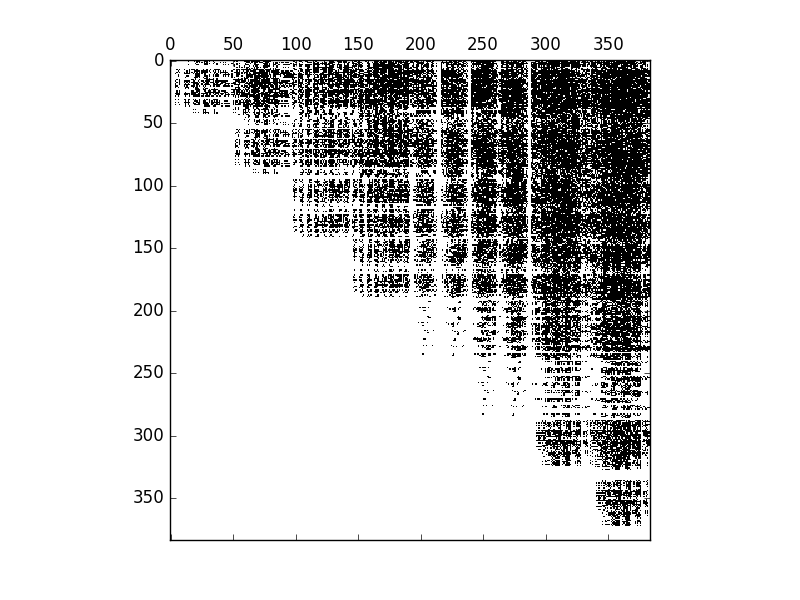
\includegraphics[width=8cm]{../png/beztri.png}
\end{center}
En appliquant à la matrice une factorisation QRP bloc après bloc, les éléments diagonaux vont alors décroitre uniquement à l'intérieur de chaque bloc, ce qui permet de préserver un saut numérique plus grand que dans la première approche. Le graphique ci dessous montre la nouvelle disposition des éléments diagonaux pour le même exemple que précédemment, traité de la deuxième façon.
\begin{center}
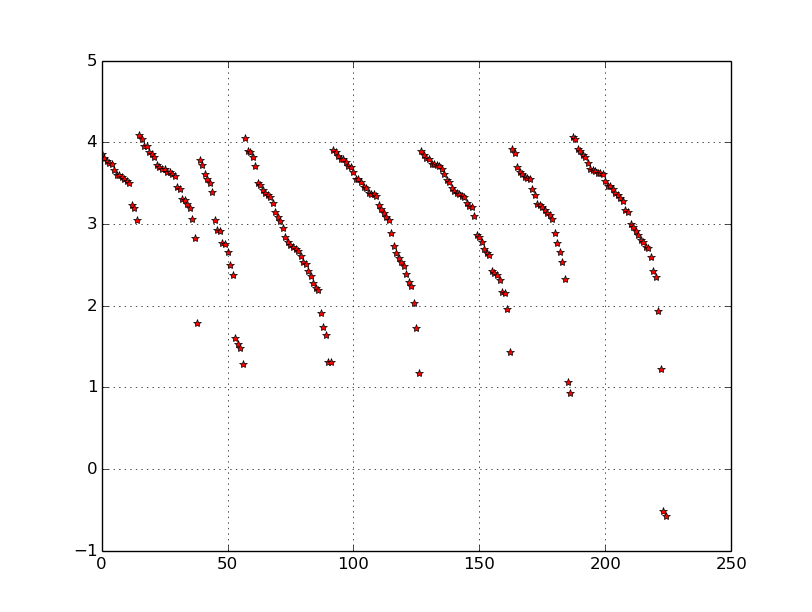
\includegraphics[width=8cm]{../png/diagRtri.png}
\end{center}
On voit que, malgré une décroissance rapide des éléments diagonaux dans chaque bloc, la plus petite taille de ceux-ci permet au plus petit élément ``non-nul" d'être beaucoup plus grand que le epsilon machine, ce qui facilite le calcul du rang numérique.

\end{document}
